\section{Appendices}
\subsection{Vada Pav}
\label{appendix:vadapav}
\begin{figure}[H]
	\centering
	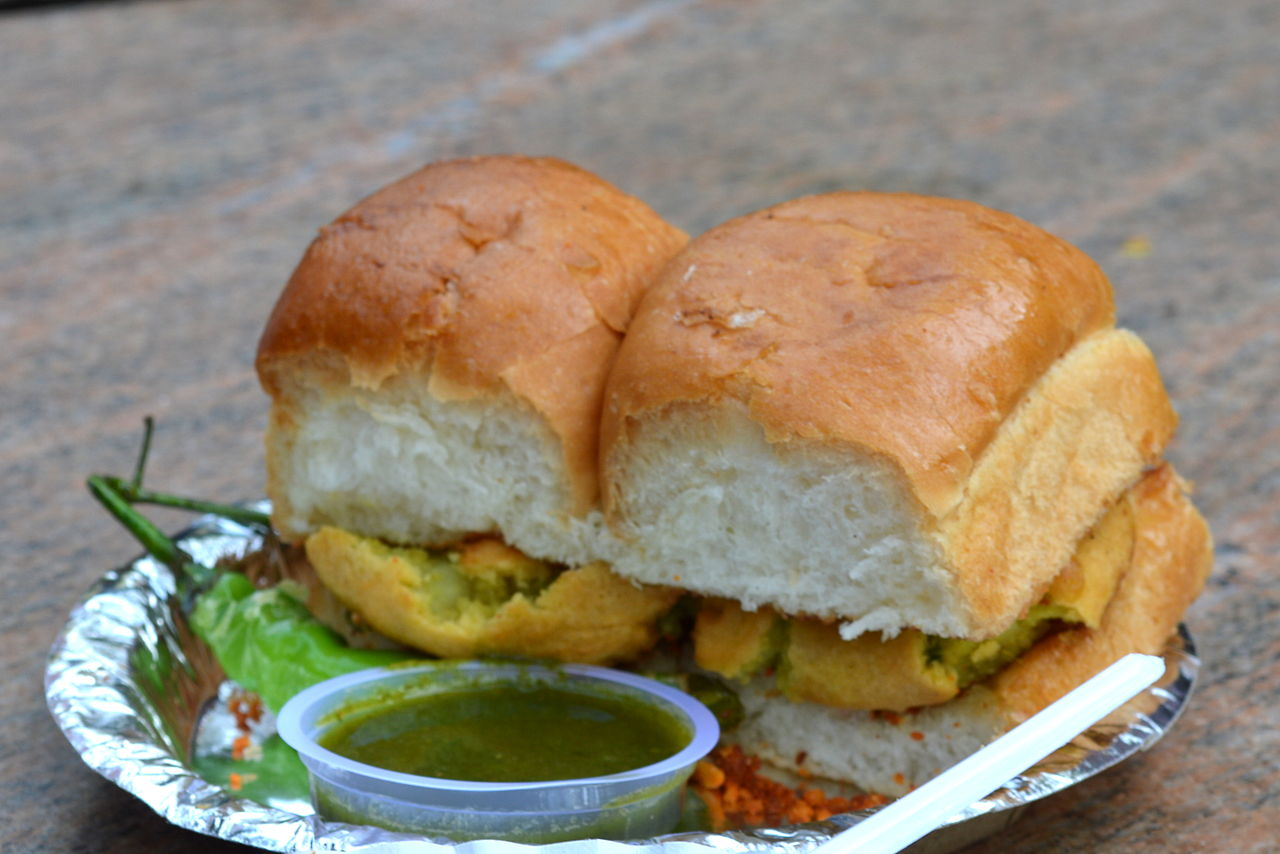
\includegraphics[height=6cm]{Figures/VadaPaav.JPG}
	\caption{Image of a vada pav used in case-based reasoning to classify a hot-dog.}
	\label{fig:vadapav}
\end{figure}

\subsection{Toast}
\label{appendix:toast}
\begin{figure}[H]
	\centering
	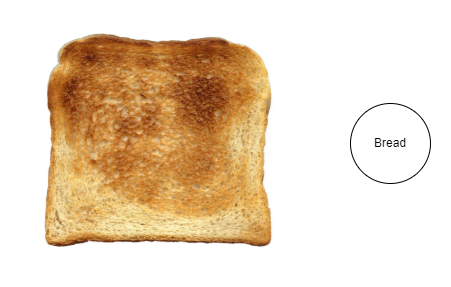
\includegraphics[height=6cm]{Figures/toast.png}
	\caption{Toast Concept Model}
	\label{fig:toast}
\end{figure}


\subsection{Ice Cream Sandwich}
\label{appendix:ics}
\begin{figure}[H]
	\centering
	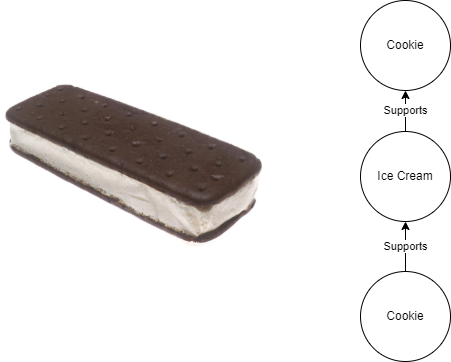
\includegraphics[height=6cm]{Figures/ice-cream-sandwich.png}
	\caption{Ice Cream Concept Model}
	\label{fig:icecream-sandwich}
\end{figure}


\subsection{Chicken Wrap}
\label{appendix:cw}
\begin{figure}[H]
	\centering
	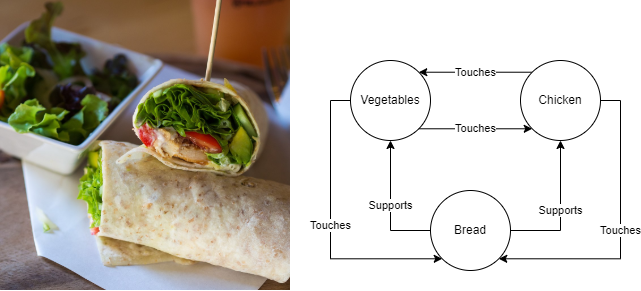
\includegraphics[height=6cm]{Figures/chicken-wrap.png}
	\caption{Chicken Wrap Concept Model}
	\label{fig:cw}
\end{figure}

\subsection{Sushi Roll}
\label{appendix:sushi}
\begin{figure}[H]
	\centering
	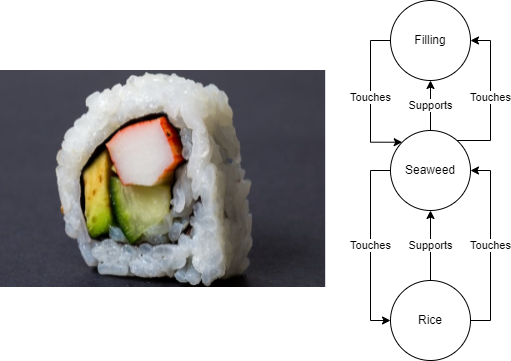
\includegraphics[height=6cm]{Figures/sushi-roll.png}
	\caption{Sushi Roll Concept Model}
	\label{fig:sushi}
\end{figure}

\subsection{Grain Background Knowledge}
\label{appendix:grain}
\begin{figure}[H]
	\centering
	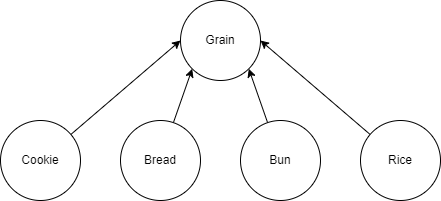
\includegraphics[height=6cm]{Figures/bg-knowledge.png}
	\caption{Background knowledge about Grains required for AI agent}
	\label{fig:bg}
\end{figure}

\subsection{Filling Background Knowledge}
\label{appendix:filling}
\begin{figure}[H]
	\centering
	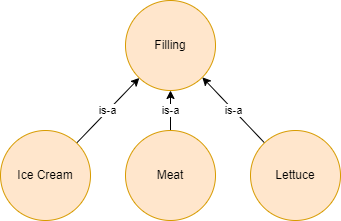
\includegraphics[height=6cm]{Figures/bg-filling-knowledge.png}
	\caption{Background knowledge about Fillings required for AI agent}
	\label{fig:bg-filling}
\end{figure}


\subsection{Plate Orientation}
\label{appendix:plate}
\begin{figure}[H]
	\centering
	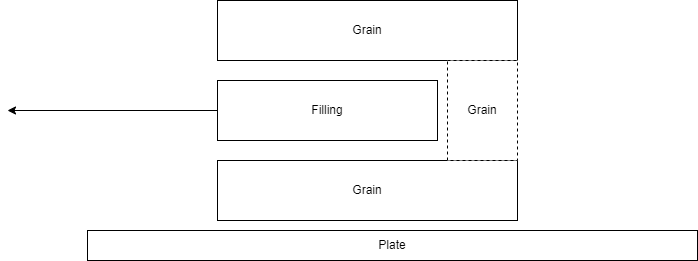
\includegraphics[height=6cm]{Figures/plane-horizontal.png}
	\caption{Diagram depicting dish and plate planes in parallel.}
	\label{fig:plate}
\end{figure}

\begin{figure}[H]
	\centering
	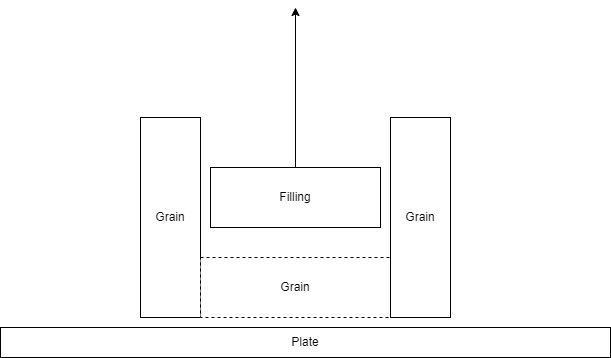
\includegraphics[height=6cm]{Figures/plane-vertical.png}
	\caption{Diagram depicting dish and plate intersection.}
	\label{fig:plate-vertical}
\end{figure}


